% !BIB TS-program = biber
% !TEX spellcheck = en_US
%---------------------------------------------------------------------------------
\documentclass[a4paper,11pt,DIV=20,BCOR=10mm] {scrartcl}
%%%%%%%%%%%%%%%%%%%%%%%%%%%%%%%%%%%%%%%%%%%%%%%%%%%%%%%%%%%%%%%%%%%%%%%%%%%%%%%%%%
\newif\ifsolution
%\solutiontrue
%%%%%%%%%%%%%%%%%%%%%%%%%%%%%%%%%%%%%%%%%%%%%%%%%%%%%%%%%%%%%%%%%%%%%%%%%%%%%%%%%%
\title{Basic Blade Design}
\subtitle{\ifsolution{\textcolor{red}{Solution of }}\fi Exercise for lecture \#1 \\ Introduction to Wind Turbine Aerodynamics}
\author{David Schlipf}
\date{17.04.2025}
%%%%%%%%%%%%%%%%%%%%%%%%%%%%%%%%%%%%%%%%%%%%%%%%%%%%%%%%%%%%%%%%%%%%%%%%%%%%%%%%%%
\def\StylePath{../WETI-Style/}
\usepackage{\StylePath/WETI-ExerciseDoc}%v1.8
\addbibresource{../WETI-Style/PublicationsDavidSchlipf.bib}
\addbibresource{../ReferencesIAWT.bib}
% Additional packages / settings
%%%%%%%%%%%%%%%%%%%%%%%%%%%%%%%%%%%%%%%%%%%%%%%%%%%%%%%%%%%%%%%%%%%%%%%%%%%%%%%%%%
\begin{document}
% ---------------------------------------
\maketitle 
% ---------------------------------------
% ---------------------------------------
\section*{Blade Design According to Betz for the NREL 5MW Wind Turbine}
% ---------------------------------------
In this exercise, blades according to Betz should be designed for the NREL 5MW Reference Wind Turbine \cite{Jonkman2009a} and compared to the original blades.
In this exercise we will use only the airfoil NACA64-A17 for the sake of simplicity. For the original blades, more airfoils are used.

Please follow the following steps
\begin{enumerate}[noitemsep,label=\alph*)] 
	\item Find the design tip speed ratio $\lambda_{\textrm{D}}$, rotor radius and number of blades in \cite{Jonkman2009a}.
	%-----
	\ifsolution{\textcolor{red}{$R=\SI{63}{m}$, $\lambda_{\textnormal{D}}=7.55$, $z=3$.}}\fi
	%=====
	\item Find useful design values for the angle of attack $\alpha_{\textrm{A}}$ and of lift coefficient $c_{\textrm{L}}$. Use the airfoil data in file \file{NACA64_A17.dat}.
	%-----
	\ifsolution{\textcolor{red}{$\alpha_{\textnormal{A}}=\SI{5}{\degree}$, $c_{\textnormal{L}}=1.011$.}}\fi
	%=====
	\item Calculate the distribution of twist angle $\beta(r)$ and of chord length $c(r)$ over the radius at the positions from the file \file{NRELOffshrBsline5MW_AeroDyn_Equil_noTwr.dat}.
	%-----
	\ifsolution{
		\newline
		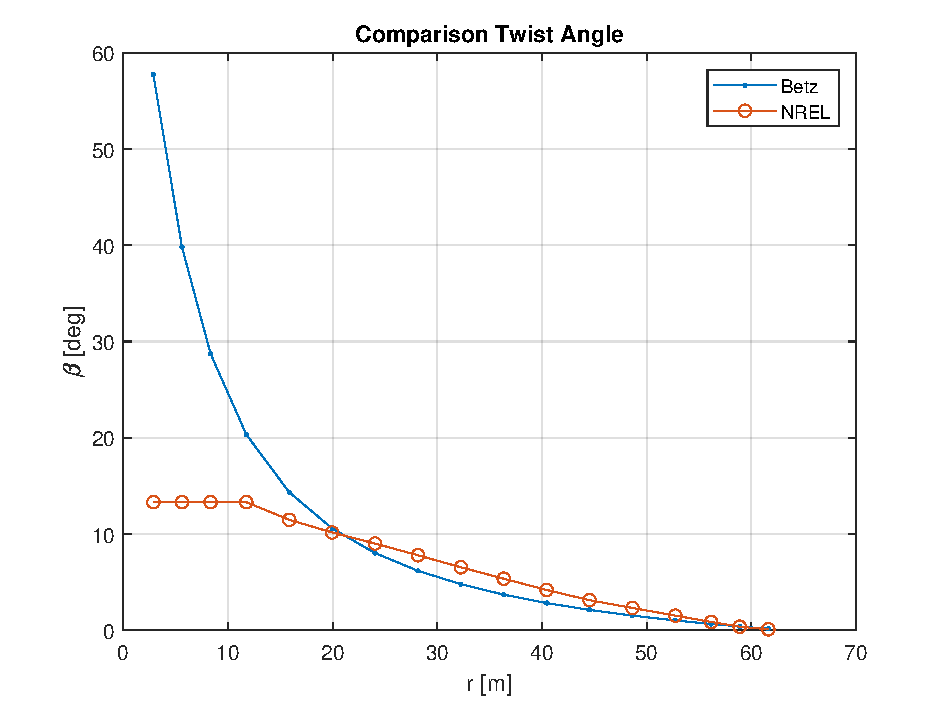
\includegraphics[width=.45\linewidth]{Figures/ComparisonTwistAngle} 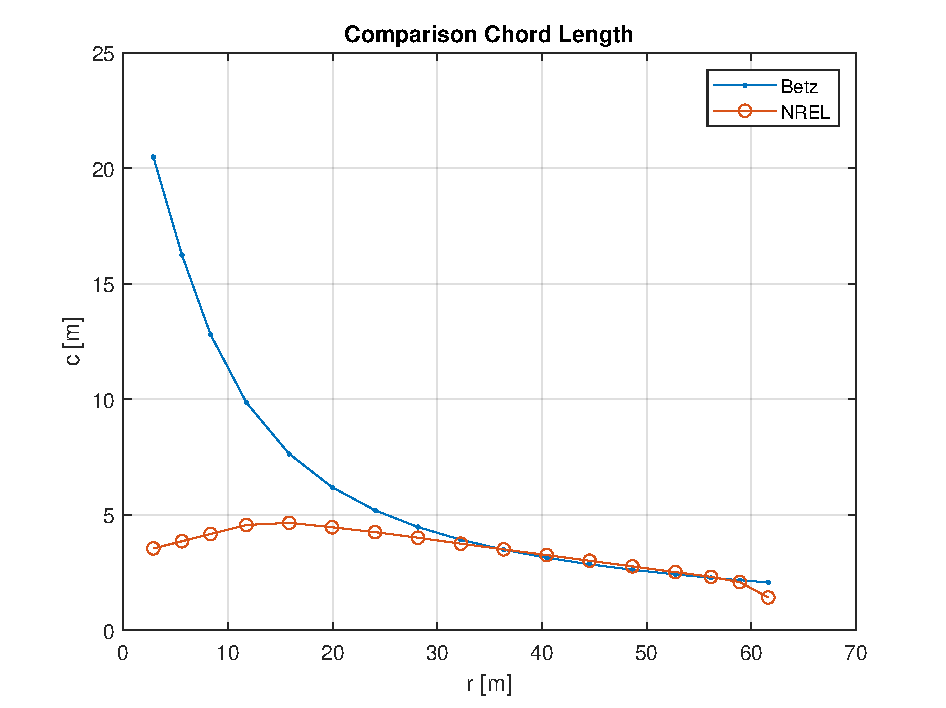
\includegraphics[width=.45\linewidth]{Figures/ComparisonChordLength} 
		\newline
		}\fi
	%=====
	\item Compare your values to the ones from the NREL design. What are the main differences?
	%-----
	\ifsolution{\textcolor{red}{Larger values for twist angle and chord length in root region.}}\fi
	%=====	
\end{enumerate}

You can use either the Matlab script \file{Exercise01.m} or the provided Excel file \file{Exercise01.xlsx}.


% bibliography
\printbibliography
\end{document}